\documentclass[aspectratio=169,10pt]{beamer}
\usetheme{Madrid}
\usecolortheme{default}

\usepackage{hyperref}
\usepackage{tikz}
\usetikzlibrary{positioning,arrows.meta}
\usepackage{amsmath,amssymb}

% --- Custom Colors ---
\definecolor{unibblue}{RGB}{0,51,102}
\definecolor{unibgold}{RGB}{212,175,55}
\definecolor{unibgreen}{RGB}{0,128,0}

\setbeamercolor{palette primary}{bg=unibblue,fg=white}
\setbeamercolor{palette secondary}{bg=unibblue!85,fg=white}
\setbeamercolor{palette tertiary}{bg=unibblue!70,fg=white}
\setbeamercolor{structure}{fg=unibblue}
\setbeamercolor{block title}{bg=unibblue!85,fg=white}
\setbeamercolor{block body}{bg=unibblue!10,fg=black}
\setbeamercolor{alertblock title}{bg=unibgold!90,fg=black}
\setbeamercolor{alertblock body}{bg=unibgold!15,fg=black}

\title{Persamaan Diferensial}
\subtitle{Minggu 7: Invers Transformasi Laplace \& Solusi PDB pada Rangkaian Elektrik}
\author{Novalio Daratha \& Muhammad Arfan}
\institute{Program Studi Teknik Elektro\\Universitas Bengkulu}
\date{2026}

\begin{document}

\begin{frame}
  \titlepage
\end{frame}

\begin{frame}{Capaian Pembelajaran (CPMK 3)}
  \begin{itemize}
    \item \textbf{CPMK 3.1:} Menguasai teknik Invers Transformasi Laplace $\mathcal{L}^{-1}\{F(s)\} = f(t)$.
    \item \textbf{CPMK 3.2:} Mampu melakukan ekspansi pecahan parsial (\textit{Partial Fraction Expansion}) untuk faktor linear, berulang, dan kuadratik irreducible.
    \item \textbf{CPMK 3.3:} Menerapkan Transformasi Laplace penuh untuk menyelesaikan PDB dan IVP sistem dinamis.
    \item \textbf{CPMK 3.4:} Menyelesaikan analisis transien rangkaian listrik menggunakan pendekatan domain-$s$ (impedansi operasional).
  \end{itemize}
\end{frame}

\begin{frame}{Daftar Isi}
  \tableofcontents
\end{frame}

\section{Metode Invers Transformasi Laplace}
\begin{frame}{Konsep Invers Transformasi Laplace}
  \begin{block}{Definisi}
    Jika $\mathcal{L}\{f(t)\} = F(s)$, maka invers transformasi Laplace didefinisikan sebagai:
    $$ {\color{unibblue} f(t) = \mathcal{L}^{-1}\{F(s)\}} $$
  \end{block}
  \pause
  \textbf{Sifat Kelinieran:}
  $$ \mathcal{L}^{-1}\{c_1 F_1(s) + c_2 F_2(s)\} = c_1 \mathcal{L}^{-1}\{F_1(s)\} + c_2 \mathcal{L}^{-1}\{F_2(s)\} $$
  \pause
  \begin{alertblock}{Strategi Praktis di Bidang Rekayasa}
    Alih-alih menghitung integral invers kompleks Bromwich, kita menguraikan rasio polinomial $F(s) = \frac{N(s)}{D(s)}$ menjadi suku-suku pecahan sederhana yang ada di tabel standar!
  \end{alertblock}
\end{frame}

\section{Ekspansi Pecahan Parsial (Partial Fractions)}
\begin{frame}{Tiga Kasus Faktor Penyebut $D(s)$}
  \begin{enumerate}
    \item \textbf{Faktor Linear Berbeda $(s - p_1)(s - p_2)$:}
    $$ \frac{N(s)}{(s-p_1)(s-p_2)} = \frac{A}{s-p_1} + \frac{B}{s-p_2} \implies f(t) = A e^{p_1 t} + B e^{p_2 t} $$
    \pause
    \item \textbf{Faktor Linear Berulang $(s - p)^n$:}
    $$ \frac{N(s)}{(s-p)^n} = \frac{A_1}{s-p} + \frac{A_2}{(s-p)^2} + \dots + \frac{A_n}{(s-p)^n} $$
    \pause
    \item \textbf{Faktor Kuadratik Kompleks $((s-\alpha)^2 + \beta^2)$:}
    $$ \frac{A(s-\alpha) + B\beta}{(s-\alpha)^2 + \beta^2} \implies f(t) = e^{\alpha t}(A \cos\beta t + B \sin\beta t) $$
  \end{enumerate}
\end{frame}

\section{Alur Lengkap Penyelesaian PDB dengan Laplace}
\begin{frame}{Diagram Alir Metode Laplace}
  \begin{center}
    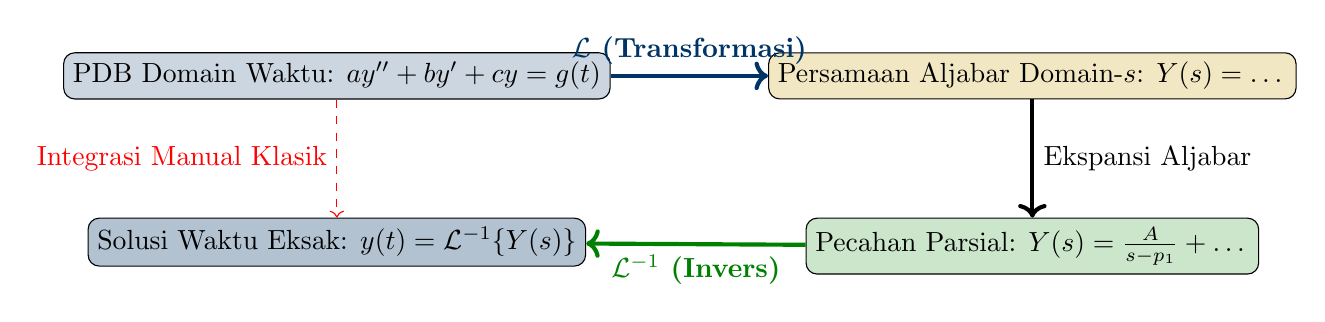
\begin{tikzpicture}[node distance=1.8cm, auto]
      \node [draw, fill=unibblue!20, rounded corners] (t_ode) {PDB Domain Waktu: $a y'' + b y' + c y = g(t)$};
      \node [draw, fill=unibgold!30, rounded corners, right=2cm of t_ode] (s_alg) {Persamaan Aljabar Domain-$s$: $Y(s) = \dots$};
      \node [draw, fill=unibgreen!20, rounded corners, below=1.5cm of s_alg] (s_frac) {Pecahan Parsial: $Y(s) = \frac{A}{s-p_1} + \dots$};
      \node [draw, fill=unibblue!30, rounded corners, below=1.5cm of t_ode] (t_sol) {Solusi Waktu Eksak: $y(t) = \mathcal{L}^{-1}\{Y(s)\}$};
      
      \draw[->, thick, line width=1.5pt, unibblue] (t_ode) -- node[above]{\textbf{$\mathcal{L}$ (Transformasi)}} (s_alg);
      \draw[->, thick, line width=1.5pt] (s_alg) -- node[right]{Ekspansi Aljabar} (s_frac);
      \draw[->, thick, line width=1.5pt, unibgreen] (s_frac) -- node[below]{\textbf{$\mathcal{L}^{-1}$ (Invers)}} (t_sol);
      \draw[dashed, ->, red] (t_ode) -- node[left]{Integrasi Manual Klasik} (t_sol);
    \end{tikzpicture}
  \end{center}
\end{frame}

\begin{frame}{Contoh Komprehensif: Penyelesaian IVP Orde 2}
  \textbf{Soal:} Selesaikan $y'' + 4y = 8e^{2t}$ dengan kondisi awal $y(0) = 0, y'(0) = 0$.
  \pause
  \begin{block}{Langkah 1: Transformasikan ke Domain $s$}
    $$ (s^2 Y(s) - s y(0) - y'(0)) + 4Y(s) = \frac{8}{s-2} $$
    $$ (s^2 + 4)Y(s) = \frac{8}{s-2} \implies Y(s) = \frac{8}{(s-2)(s^2 + 4)} $$
  \end{block}
  \pause
  \begin{block}{Langkah 2: Pecahan Parsial}
    $$ \frac{8}{(s-2)(s^2 + 4)} = \frac{A}{s-2} + \frac{B s + C}{s^2 + 4} $$
    Samakan pembilang: $8 = A(s^2 + 4) + (Bs + C)(s-2)$.
    \begin{itemize}
      \item Untuk $s = 2$: $8 = A(8) \implies A = 1$.
      \item Samakan koefisien $s^2$: $A + B = 0 \implies B = -1$.
      \item Samakan konstanta: $4A - 2C = 8 \implies 4(1) - 2C = 8 \implies C = -2$.
    \end{itemize}
  \end{block}
\end{frame}

\begin{frame}{Langkah 3: Invers Transformasi ke Domain Waktu}
  $$ Y(s) = \frac{1}{s-2} - \frac{s + 2}{s^2 + 4} = \frac{1}{s-2} - \frac{s}{s^2 + 2^2} - \frac{2}{s^2 + 2^2} $$
  \pause
  Terapkan tabel invers standar:
  \begin{alertblock}{Solusi Khusus PDB}
    $$ {\color{unibblue} y(t) = e^{2t} - \cos(2t) - \sin(2t)} $$
  \end{alertblock}
  \textit{Catatan: Kondisi awal $y(0)=0$ dan $y'(0)=0$ sudah otomatis terbukti!}
\end{frame}

\section{Aplikasi Rangkaian Elektrik}
\begin{frame}{Analisis Rangkaian dengan Impedansi Kompleks $s$}
  \begin{table}[]
    \centering
    \begin{tabular}{|c|c|c|}
      \hline
      \textbf{Komponen} & \textbf{Hubungan Waktu $t$} & \textbf{Impedansi Laplace $Z(s)$} \\ \hline
      Resistor ($R$) & $v(t) = R i(t)$ & $Z_R(s) = R$ \\ \hline
      Induktor ($L$) & $v(t) = L \frac{di}{dt}$ & $Z_L(s) = sL$ (dengan sumber $L i(0)$) \\ \hline
      Kapasitor ($C$) & $i(t) = C \frac{dv}{dt}$ & $Z_C(s) = \frac{1}{sC}$ (dengan sumber $\frac{v(0)}{s}$) \\ \hline
    \end{tabular}
  \end{table}
  \pause
  Hukum Ohm Domain-$s$: $V(s) = I(s) \cdot Z(s)$.
\end{frame}

\begin{frame}{Rangkuman Materi Minggu 7}
  \begin{enumerate}
    \item Transformasi Laplace mengubah proses turunan kalkulus menjadi manipulasi pecahan aljabar.
    \item Kondisi awal dimasukkan langsung di langkah awal perumusan.
    \item Ini merupakan metode fondasi dalam teori sistem kendali (\textit{Control Systems}) dan analisis rangkaian elektrik transien.
  \end{enumerate}
\end{frame}

\end{document}
